\documentclass[11pt,a4paper]{exam}
\usepackage[utf8]{inputenc}
\usepackage{graphicx}
\usepackage{amsmath}
\usepackage{array}
\usepackage{geometry}
\usepackage{tikz}
\usepackage{enumitem}
\usepackage{booktabs}

% Set page margins for single page
\geometry{left=1.5cm, right=1.5cm, top=1.5cm, bottom=1.5cm}

% Header formatting
\header{National Institute of Technology Calicut}{}{Blockchain Technology Examination}
\footer{}{\thepage}{}
\headheight 1cm
\footskip 1cm

% Question formatting - changed to show marks instead of points
\qformat{\textbf{Question \thequestion}\hfill}

% Define custom commands
\newcommand{\examdate}{September 19, 2025}
\newcommand{\maxmarks}{25}
\newcommand{\timeduration}{1 hour}

\begin{document}

\begin{center}
\large \textbf{National Institute of Technology Calicut} \\
\large \textbf{Department of Computer Science and Engineering} \\
\vspace{0.3cm}
\Large \textbf{Blockchain Technology Examination} \\
\vspace{0.3cm}
\normalsize
\begin{tabular}{|p{0.3\textwidth}|p{0.3\textwidth}|}
\hline
\textbf{Maximum Marks:} \maxmarks & \textbf{Time Duration:} \timeduration \\
\hline
\textbf{Date:} \examdate & \textbf{Academic Year:} 2025-2026 \\
\hline
\end{tabular}
\end{center}

\vspace{0.3cm}
\textbf{Instructions:}
\begin{itemize}
\item Attempt all questions.
\item Draw neat diagrams wherever required.
\end{itemize}

\vspace{0.3cm}
\begin{questions}

% Question 1 - Multiple Choice (2 questions)
\question[4] \textbf{Multiple Choice Questions:} \hfill \textbf{(4 marks)}
\begin{enumerate}
\item Which cryptographic concept is fundamental to blockchain technology?
\begin{oneparchoices}
\choice Symmetric encryption
\choice Hash functions
\choice Steganography
\choice Quantum cryptography
\end{oneparchoices}

\item What is the primary purpose of a consensus mechanism in blockchain?
\begin{oneparchoices}
\choice To increase transaction speed
\choice To validate and agree on transactions
\choice To create new cryptocurrencies
\choice To reduce energy consumption
\end{oneparchoices}
\end{enumerate}

% Question 2 - Diagram-based with embedded diagram
\question[5] Study the following blockchain structure diagram and answer the questions below: \hfill \textbf{(5 marks)}

\begin{center}
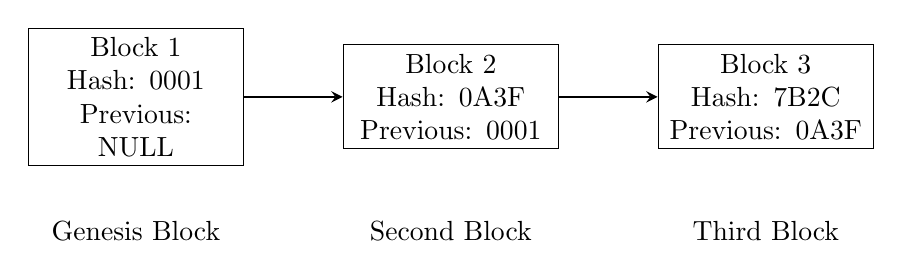
\begin{tikzpicture}[
    block/.style={rectangle, draw, text width=2.5cm, minimum height=1cm, text centered},
    arrow/.style={thick, ->, >=stealth}
]

% Blocks
\node[block] (block1) at (0,0) {Block 1 \\ Hash: 0001 \\ Previous: NULL};
\node[block] (block2) at (4,0) {Block 2 \\ Hash: 0A3F \\ Previous: 0001};
\node[block] (block3) at (8,0) {Block 3 \\ Hash: 7B2C \\ Previous: 0A3F};

% Arrows
\draw[arrow] (block1.east) -- (block2.west);
\draw[arrow] (block2.east) -- (block3.west);

% Labels
\node[below of=block1, yshift=-0.7cm] {Genesis Block};
\node[below of=block2, yshift=-0.7cm] {Second Block};
\node[below of=block3, yshift=-0.7cm] {Third Block};

\end{tikzpicture}
\end{center}

\begin{enumerate}
\item What is the purpose of the "Previous" field in each block?
\item If an attacker tries to modify data in Block 1, what would happen to the hashes in subsequent blocks?
\end{enumerate}

% Question 3 - Equation-based
\question[5] The Proof of Work consensus algorithm can be represented by the equation: \hfill \textbf{(5 marks)}
\[
H(nonce || block\ data) < target
\]
Explain what each component of this equation represents and how it ensures blockchain security.

% Question 4 - Table-based with embedded table
\question[5] Based on the following table comparing public and private blockchains: \hfill \textbf{(5 marks)}

\begin{center}
\begin{tabular}{|l|c|c|}
\hline
\textbf{Feature} & \textbf{Public Blockchain} & \textbf{Private Blockchain} \\
\hline
Access Control & Anyone can join & Permissioned \\
\hline
Transaction Speed & Slower (5-15 TPS) & Faster (100-1000 TPS) \\
\hline
Consensus & PoW/PoS & Voting-based \\
\hline
Use Cases & Cryptocurrency & Supply chain \\
\hline
\end{tabular}
\end{center}

Answer the following:
\begin{enumerate}
\item Which type of blockchain would be more suitable for a banking system? Why?
\item What is the main trade-off between transaction speed and decentralization?
\end{enumerate}

% Question 5 - Matrix-based
\question[6] In blockchain networks, transaction verification can be represented using matrices: \hfill \textbf{(6 marks)}
\[
V = \begin{bmatrix}
1 & 0 & 1 \\
0 & 1 & 1 \\
1 & 1 & 0 \\
\end{bmatrix}
\]
A value of 1 indicates verification by that node. If the consensus rule requires at least 2 verifications per transaction, which transactions would be accepted? Show your calculations.

\end{questions}

\vspace{0.5cm}
\begin{center}
\textbf{END OF QUESTION PAPER}
\end{center}

\end{document}